\chapter{Background}

In this chapter, we will present the relevant background information.

\section{Categories of Recommender Systems}
To better understand how our work fits into the research field of recommendations, we first want to explain the different types of recommender systems.

One typically classifies recommender systems into three categories.
Collaborative recommenders, content-based recommenders, and sequential recommenders~\cite{melville2010recommender}.

\subsection{Collaborative Recommender Systems}
Collaborative recommender systems focus on similarities between users based on their preferences. At first, users get assigned different weights based on similarity to other users. Neighborhood methods are used to find the nearest neighbors of a particular user with the highest similarity scores. We can then recommend items to the user that similar users have liked in the past. This method completely ignores the content of items.

\subsection{Content-based Recommender Systems}
Content-based recommender systems only focus on the content and features of items. The goal is to recommend items similar to items the user has interacted with in the past. By learning about the content of items, the system can then make recommendations. The content is often textual for example a review of a movie, a description of a video, or a social media post. Content is then converted into some vector representation. Given the vectors, we can calculate the similarity between items and recommend an item to the user that is similar to the items she has interacted with in the past.

\subsection{Sequential Recommender Systems}
In this work, we want to concentrate on sequential recommender systems, which have become popular in academia and the industry in recent years. Conventional recommender systems like collaborative and content-based recommenders can only model user preferences statically. In contrast, sequential recommender systems model sequential dependencies of interactions between a user and items to issue recommendations~\cite{wang2019survey, wang2019sequential}. The items a user interacts with are not isolated. Recent purchases can affect the current decisions. They are also affected by the user's preferences which change over time. This phenomenon is often referred to in the literature as concept drift~\cite{tsymbal2004problem}. We can observe concept drift in two different forms. A gradual change over time, for example, seasonal changes in weather predictions. But also sudden changes such as a breaking news event that influences the behavior of users. Traditional models are not well equipped to handle the change over time. Taking the sequential order of interactions into account when we make recommendations seems natural and has inspired the development of sequential recommender systems.

Existing work typically falls into one of the three categories.
In our work, we will combine two sequential recommender systems into a hybrid design. Our system will encode arbitrary content to capture the full expressivity of the data and adapt its attention based on changes in the data.


\section{Ensemble Learning}
\label{sec:ensemble_learning}

The "wisdom of the crowd" is a phenomenon that shows the aggregated answers to a complex question from a large group of random individuals are often better than the answer of a single expert. This type of crowd effect has been empirically shown in several experiments where people had to make numerical estimations~\cite{yi2012wisdom}. Luckily, one can apply the same idea to machine learning.

A group of different machine learning models is often called an ensemble. Ensemble learning is an active research area that explores how we can effectively combine models to get more accurate predictions. There are several reasons why ensemble learning is powerful~\cite{dietterich2000ensemble}.

The first reason is computational. Machine learning models often perform gradient descent to minimize an error function. Unfortunately, gradient descent does not always converge to the global optimum. Instead, gradient descent can get stuck in a local optimum. An ensemble of models may provide a more accurate approximation considering each model can search for the optimum from a different starting point.

The second reason is statistical. We can look at a machine learning model as a search space with an optimal hypothesis. In statistics, the law of large numbers states, that if we conduct an experiment a large number of times and take the average, the result will converge to the ground truth~\cite{ibe2013markov}. We can exploit this law by expanding the amount of data we train with and by training multiple models. 

\subsection{Stacking}
Stacking is an ensemble method that aggregates the outputs of several models~\cite{geron2019hands}. In the context of recommender systems, we can fuse the output probabilities by taking a weighted average, a majority voting, or by using the maximums of the probabilities across the models. With the help of a hold-out set and meta-learning, the system learns to give different weights to the models for maximum accuracy.

\subsection{Boosting}
Boosting is an ensemble method where models are combined sequentially~\cite{geron2019hands}. The output of each model gets passed on to the next model. That way, each model tries to correct the predictions of the previous model. In our case, we can drop items with a low probability as they pass through the chain of models so that subsequent models have a reduced sample size of items to make predictions.


\section{Standard Evaluation Metrics}\label{sec:standard_metrics}

As we will describe in the Section~\nameref{sec:test_procedure}, we feed the system 100 negative items that the user has not engaged with, plus the test set item (the last item in the user’s sequence). To demonstrate the calculation of our metrics, we have created an illustration in Figure~\ref{fig:illustration_metrics} that shows the prediction output for three random users.

\begin{figure}[htbp]
\centering
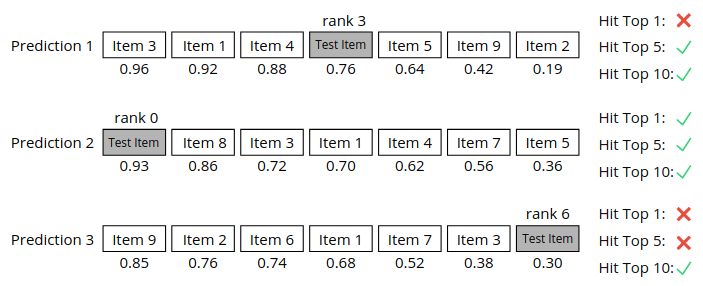
\includegraphics[width=0.95\textwidth]{images/illustrations/metrics.png}
\caption{Example illustration for the computation of our metrics for three random predictions}
\label{fig:illustration_metrics}
\end{figure}

Our models use a softmax output layer which gives us a probability distribution over all the items. Each item gets a probability of being the last item in the user's sequence, and all probabilities sum up to 1. Items are then ordered by probability and ranked. The item with the highest probability gets a rank of 0. Finally, we need the rank of the actual last item, the test item, to compute our metrics.


\paragraph{Hit Rate:}
Our primary metric is the hit rate. To calculate the hit rate, we check the ratio of how many times the test set item was in the top n predictions. A higher hit rate indicates a better accuracy. Our example in Figure~\ref{fig:illustration_metrics} yields the following hit rates:

\begin{equation}
\setlength{\jot}{25pt}
    \begin{aligned}
        hit rate @1=\frac{\text{\# Hit Top 1}}{\text{\#Predictions}}=\frac{1}{3}\approx0.33 \\
        hit rate @5=\frac{\text{\# Hit Top 5}}{\text{\#Predictions}}=\frac{2}{3} \approx 0.66\\
        hit rate @10=\frac{\text{\# Hit Top 10}}{\text{\#Predictions}}=\frac{3}{3}=1.0 
    \end{aligned}
    \label{equation:hit_rate}
\end{equation}

\paragraph{Normalized Discounted Cumulative Gain (NDCG):}
To calculate the NDCG, we sum up the inverse logarithmic ranks and normalize, by dividing the result by the number of total predictions. We can determine the NDCG@n by summing up only test set items positioned in the top n predictions. A higher NDCG indicates more accurate predictions. For our example in Figure~\ref{fig:illustration_metrics}, we get the following NDCG scores:

\begin{equation}
\setlength{\jot}{25pt}
    \begin{aligned}
        NDCG@n&=\frac{ \sum\limits_{rank<n}
      \frac{1}{log_2(rank + 2)}}
      {\text{\#Predictions}} \\
        NDCG@1&=\frac{\frac{1}{log_2(0 + 2)}}{3}\approx 0.33 \\
        NDCG@5&=\frac{\frac{1}{log_2(0 + 2)}+\frac{1}{log_2(3+2)}}{3}\approx 0.48 \\
        NDCG@10&=\frac{\frac{1}{log_2(0 + 2)}+\frac{1}{log_2(3+2)}+\frac{1}{log_2(6+2)}}{3}\approx 0.59
    \end{aligned}
    \label{equation:NDCG}
\end{equation}


\paragraph{Mean Average Precision (MAP):}
The Mean Average Precision is the sum of all the inverse ranks divided by the number of predictions. Figure~\ref{fig:illustration_metrics} would give us the following score:

\begin{equation}
\setlength{\jot}{25pt}
    \begin{aligned}
        MAP=\frac{ \sum\limits_{rank}
      \frac{1}{rank + 1}}
      {\text{\#Predictions}} = \frac{\frac{1}{0+1} +\frac{1}{3+1} + \frac{1}{6+1}}{3} \approx 0.46
    \end{aligned}
    \label{equation:MAP}
\end{equation}